% Edgar Fournival <contact@edgar-fournival.fr>

\documentclass[12pt,a4paper]{report}

\usepackage[francais]{babel}
\addto\captionsfrench{\renewcommand{\chaptername}{Partie}}

\usepackage{ifxetex}

\ifxetex
	\usepackage{fontspec}
\else
	\usepackage[T1]{fontenc}
	\usepackage[utf8]{inputenc}
\fi

\usepackage{amsmath}
\usepackage{amssymb}
\usepackage{eurosym}
\usepackage{mathtools}

\usepackage[noend]{algorithmic}
\renewcommand{\algorithmicif}{\textbf{si}}
\renewcommand{\algorithmicthen}{\textbf{alors}}
\renewcommand{\algorithmicfor}{\textbf{pour}}
\renewcommand{\algorithmicdo}{\textbf{faire}}

\usepackage{enumitem}
\usepackage{adjustbox}
\usepackage[hidelinks,breaklinks]{hyperref}
\usepackage[bottom]{footmisc}
\usepackage[justification=centering]{caption}
\usepackage{float}
\usepackage{graphicx}
\usepackage{tikz}
\usetikzlibrary{arrows,decorations.pathreplacing}

\usepackage{chngcntr}
\counterwithout{figure}{chapter}

\usepackage{csquotes}
\usepackage[backend=biber,sortcites,sorting=nty,backref,natbib,hyperref,url=false,doi=false]{biblatex}
\addbibresource{rapport.bib}

\interfootnotelinepenalty=10000
\usepackage[bottom]{footmisc}

\setlength\parindent{1.5em}
\setlength\parskip{0.3em}

\usepackage{tocloft}
\setlength\cftbeforetoctitleskip{3em}

\makeatletter
\g@addto@macro \normalsize {
	\setlength{\abovedisplayskip}{0.25em}
	\setlength{\belowdisplayskip}{0.25em}
}
\makeatother

\let\emptyset\varnothing
\let\leq\leqslant
\let\geq\geqslant

\renewcommand{\thechapter}{\Roman{chapter}}
\newcommand{\gen}[1]{\left<#1\right>}
\newcommand{\sgnode}[1]{{\bf \left<#1\right>}}
\newcommand{\gr}[1]{{\color{gray} #1}}

\usepackage{titlepic}

\title{\bfseries\LARGE TER individuel\\[0.5em]\Huge Distribution d'un calcul combinatoire}
\author{\bfseries\Large Edgar Fournival}
\date{}

\titlepic{
	\vskip 5em
	{\Large Encadrant : Florent Hivert}\\[2em]
	
\includegraphics[height=3.5cm,keepaspectratio]{logo-lri.jpg}
	\hspace{1em}
	
\includegraphics[height=3.6cm,keepaspectratio]{logo-upsud.jpg}
}

\begin{document}

\maketitle

\tableofcontents

\chapter*{Introduction}
\addcontentsline{toc}{chapter}{Introduction}

Dans le cadre du deuxième semestre du M1 Informatique de Paris-Saclay se déroulant à l'Université Paris-Sud, une unité d'enseignement de TER est proposé aux étudiants. L'acronyme TER signifie Travail d'Études et de Recherche, il peut être réalisé de manière individuelle au sein d'un laboratoire de Paris-Saclay ou en groupe à travers les différents sujets proposés en début de semestre. Aucun des sujets proposés ne m'intéressait réellement. De plus, j'ai trouvé qu'un TER individuel était une bonne opportunité d'approfondir l'aspect recherche de ma formation.

J'ai donc contacté Florent Hivert, qui était responsable du cours d'algorithmique l'année dernière en L3 MIAGE apprentissage, afin de savoir si un encadrement individuel était possible. Sa réponse fût positive et nous nous sommes rencontrés afin de discuter de la mission et des modalités. C'est comme cela que j'ai effectué mon TER au LRI au sein de l'équipe GALaC. Le sujet porte sur la distribution d'un calcul combinatoire, plus précisément l'exploration de l'arbre de semigroupes numériques. J'ai ainsi été confronté à un problème combinatoire s'inscrivant tout à fait dans le programme du M1 Informatique, notamment en continuité de la matière Algorithmique Avancée.

Dans ce rapport, je vais tout d'abord présenter le contexte de ce TER puis dans un deuxième temps expliquer plus en détails le problème posé et la solution existante. J'évoquerai enfin les développements effectués pour le distribuer et les résultats obtenus.

\chapter{Contexte}

\section{Laboratoire et équipe de recherche}

J'ai réalisé ce TER au Laboratoire de Recherche en Informatique (LRI) présent sur le campus d'Orsay. Il s'agit d'une unité mixte de recherche (UMR 8623) menée conjointement par l'Université Paris-Sud et le CNRS.

Ma mission s'est déroulée dans le bâtiment 650 Ada Lovelace, qui héberge aussi des enseignants chercheurs de l'Inria.

\begin{figure}[h]
	\centering
	
\includegraphics[scale=0.2]{logo-odk.png}
	\caption{Le logo d'OpenDreamKit}
\end{figure}

Plus précisément, j'ai été accueilli au sein de l'équipe GALaC (Graphes, Algorithmes et Combinatoire) à laquelle appartient mon enseignant encadrant. Dirigée par Johanne Cohen, cette équipe de recherche travaille sur des problématiques de calcul algébrique, d'algorithmique, de théorie des graphes ou encore sur la spécification théorique de systèmes en réseau.

L'équipe GALaC participe activement au développement de Sage. Il s'agit d'un ensemble de bibliothèques avec une interface en Python permettant de fournir des outils communs aux mathématiciens. Pour soutenir ce développement, Nicolas Thiéry est coordinateur du projet Horizon 2020 OpenDreamKit\footnote{\url{http://opendreamkit.org/}}.

Cet effort de mutualisation des développements est commun à une dizaine d'universités européennes. Il permet de concentrer les efforts de 50 personnes réparties dans 16 sites sur la maintenance de librairies utilisées par Sage. Le budget total du projet est de 7.6 millions d'euros et sert en majeure partie à employer 11 chercheurs (en moyenne) à temps plein pour travailler sur OpenDreamKit.

\section{Mission}
Mon travail a consisté à distribuer un calcul combinatoire sur plusieurs machines. Il s'agit de compter le nombre de semigroupes numériques par exploration d'arbre jusqu'à une profondeur donnée.

Cette mission s'inscrit dans le livrable 5.6 de la proposition OpenDreamKit cadrant notamment l'infrastructure et les besoins liés aux calculs efficaces en combinatoire. En effet, cela permet notamment d'approfondir et de développer des techniques d'exploration d'arbres fortement déséquilibrés.

L'algorithme mis en \oe{}uvre dans cet TER a été proposé et implémenté par Florent Hivert et Jean Fromentin, de l'Université du Littoral Côte d'Opale. Il est implémenté en \texttt{C++} et fait appel à de nombreuses techniques pour réduire le temps de calcul : vectorisation, parallélisation à l'aide de la bibliothèque \texttt{Cilk++}, dérécursivation de l'exploration, optimisations des boucles et des accès mémoire ainsi qu'un choix rigoureux des types de données.

La principale limite de cette implantation est qu'il n'est pas possible de le distribuer facilement sur plusieurs machines. L'arbre d'exploration n'étant pas équilibré, des problèmes de charge se posent rapidement. En effet, au bout d'un certain temps, une seule machine voire un seul c\oe{}ur finit par réaliser tout le travail. L'équilibrage entre plusieurs c\oe{}urs à été mis en place très simplement et de manière performante à l'aide de la librairie Intel Cilk Plus\footnote{\url{https://www.cilkplus.org/}} qui travaille en mémoire partagée. Une solution possible à ce déséquilibrage serait la mise en place d'un système de vol de tâches, non plus limité à l'échelle du processeur, mais étendu à l'échelle d'une multitude de machines.

Le but de ce TER est donc de fournir une solution pour le calcul du nombre de semigroupes qui est performante, parallélisée et surtout distribuée. L'objectif à terme sera de lancer le calcul final sur un \emph{cluster} de machines à hautes performances.

\section{Organisation}
Le travail sur ce TER a été effectué en autonomie avec un créneau d'une journée par semaine au LRI pour faire le point sur les tâches à effectuer et résoudre les difficultés.

Les horaires sont assez flexibles et je constate que la stratégie mise en place ici se fonde d'avantage sur le travail effectué que sur des heures fixes à respecter. Le télétravail est tout à fait intégré au fonctionnement de l'équipe. Il s'agit d'un mode de travail que j'ai déjà expérimenté lorsque j'étais apprenti et j'en étais très satisfait.

Tout au long de ce TER, j'ai travaillé de manière graduelle en testant et en expérimentant divers algorithmes ou techniques qui ont finalement permis de réaliser le programme final. Par exemple, j'ai commencé par implémenter dans le langage cible l'algorithme de calcul que nous souhaitions distribuer. Après nous être assuré des performances et de son fonctionnement, j'ai effectué des tests de concurrence avant de continuer.

J'ai noté mon avancement au fur et à mesure et un compte-rendu par période est visible en annexe \ref{anx:deroulement}.

Au final, l'objectif durant ce TER était de réaliser un programme permettant de distribuer le calcul et de le lancer avant la fin de ma mission. Ayant eu beaucoup de travail le dernier mois de mon année universitaire, cela a pris du retard. Nous avons aussi été confrontés à un bogue dans le compilateur GCC dont l'analyse et l'isolation a pris du temps. J'espère néanmoins pouvoir démarrer l'expérimentation avant la soutenance.

\chapter{Problème posé}

\section{Modélisation}
L'exploration de l'arbre d'un semigroupe numérique n'est pas triviale et est apparentée au problème de Frobenius. Le mathématicien Georg Frobenius s'est en effet posé la question suivante : quel est le montant maximal que l'on peut pas rendre en fonction de pièces de monnaie données ?

Ce montant se nomme ``nombre de Frobenius'' et est plus formellement décrit par le plus grand entier qu'il est impossible de calculer à partir de coefficients donnés. On peut aussi visualiser ce problème en considérant les scores au Rugby : quels sont les scores que l'on ne peut pas obtenir avec le but (3 points), l'essai (5 points) et l'essai transformé (7 points) ?

La résolution des scores au Rugby est simple, on ne peut pas avoir 1, 2 ou 4 points; tous les autres scores sont possibles. En effet, il est aisé de calculer le nombre de Frobenius (ici, 4) pour $n \leq 3$ où $n$ est le nombre d'entiers possibles pour la combinaison. Ici, $n = 3$ pour $\{3,5,7\}$.

Dans notre problème, on veut calculer le nombre de semigroupes numériques (aussi appelé monoïdes) différents jusqu'à un genre maximum donné. Un semigroupe numérique est composé de générateurs, il s'agit d'un ensemble minimal de nombres qu'on ne peut pas obtenir en combinant d'autres nombres appartenant au monoïde. Ces combinaisons (au moins une addition) sont appelées décompositions, si pour un nombre du semigroupe il y a une et une seule décomposition alors ce nombre est un générateur.

Le genre d'un semigroupe numérique correspond à sa profondeur dans l'arbre et aussi au nombre de ``trous''. On appelle trou un générateur qui a été enlevé.

Le nombre de Frobenius d'un semigroupe est la valeur du plus grand trou.

Le conducteur est le nombre à partir duquel le nombre de décompositions est d'au moins 2.

En retirant des nombres générateurs aux semigroupes numériques, on obtient un arbre très déséquilibré que nous voulons explorer.

\begin{figure}[h]
	\makebox[\textwidth][c]{\begin{tikzpicture}[scale=1.2,level distance=2cm, inner sep=2mm,level/.style={sibling distance=1.55cm}]
		\node {$\sgnode{1}$}
		child {node {$\sgnode{2,3}$}
			child [sibling distance=4.5cm] {node {$\sgnode{3,4,5}$}
	child {node {$\sgnode{4,5,6,7}$}
		child [sibling distance=2cm]{node {$\sgnode{5,6,7,8,9}$}	edge from parent node [left] {4}}
		child [sibling distance=1.9cm]{node {$\sgnode{\gr 4,6,7,9}$}	edge from parent node [left] {5}}
		child {node {$\sgnode{\gr 4,\gr 5,7}$}	edge from parent node [right] {6}}
		child {node {$\sgnode{\gr 4,\gr 5,\gr 6}$}	edge from parent node [right] {7}}
		edge from parent node [left] {3}
	}
	child{{} edge from parent[draw=none]}
	child{{} edge from parent[draw=none]}
	child {node {$\sgnode{\gr 3,5,7}$}
		child {node {$\sgnode{\gr 3,7,8}$} edge from parent node [left] {5}}
		child {node {$\sgnode{\gr 3,\gr 5}$} edge from parent node [right] {7}}
		edge from parent node [left] {4}
	}
	child {node {$\sgnode{\gr 3,\gr 4}$}
		edge from parent node [right] {5}
	}
	edge from parent node [left] {2}
			}
			child [sibling distance=4.5cm] {node {$\sgnode{\gr2,5}$}
	child {node {$\sgnode{\gr2,7}$}
		child {node {$\sgnode{\gr2,9}$}
			edge from parent node [right] {7}
		}
		edge from parent node [right] {5}
	}
	edge from parent node [right] {3}
			}
			edge from parent node [left] {1}
		}
		;
	\end{tikzpicture}}
	\caption{Les 4 premiers étages de l'arbre des semigroupes numériques (les générateurs retirés sont spécifiés sur les arêtes), selon Florent Hivert et Jean Fromentin \cite{exploring-ns}}
\end{figure}

\section{Un exemple}
Prenons un semigroupe numérique quelconque noté $S_X$ où $X$ est le genre :
\[ S_8 = \{0, \mathbf{6}, \mathbf{7}, \mathbf{10}, \mathbf{15}, 16, 17\} \cup [18; +\infty[ \]

L'ensemble minimal de \textbf{nombres générateurs} a été mis en gras, on constate qu'on peut générer tous les autres nombres à partir de ceux-ci.

Le \textbf{genre} est égal à 8 car il y a huit trous, c'est à dire que pour 8 nombres, le nombre de décompositions est nul. Si on place ce semigroupe numérique dans un arbre, il aurait une profondeur de 8 également.

Voici les 18 premiers nombres de décompositions de ce monoïde :

{\centering \vskip 0.3em
	\begin{tabular}{|*{18}{c|}}
		\hline
		0 & 1 & 2 & 3 & 4 & 5 & \textbf{6} & \textbf{7} & 8 & 9 & \textbf{10} & 11 & 12 & 13 & 14 & \textbf{15} & 16 & 17 \\
		\hline
		1 & 0 & 0 & 0 & 0 & 0 & 1 & 1 & 0 & 0 & 1  & 0  & 2  & 2  & 2  & 1  & 2  & 2  \\
		\hline
	\end{tabular}
\par \vskip 0.3em}

La \textbf{multiplicité} est de 11, soit le plus grand nombre dont le nombre de décompositions est nul.

Le \textbf{nombre de Frobenius} de ce semigroupe est égal à 15, soit le plus grand générateur.

Le \textbf{conducteur} est 16 (suivant le Frobenius), tous les nombres à partir de celui-ci peuvent être générés d'au moins deux manières :
\begin{itemize}
	\item	l'ajout de zéro au nombre, soit $0 + 16$ (ou $16 + 0$, mais on va ignorer la commutativité)
	\item	la somme de deux nombres générateurs, ici $6 + 10$
\end{itemize}

Ce monoïde va en engendrer un autre si on retire, par exemple, 15 :
\[ S_9 = \{ 0, \mathbf{6}, \mathbf{7}, \mathbf{10}, 11 \} \cup [12; +\infty[ \]

Dans la suite du rapport, le semigroupe numérique présenté ci-dessus pourra être noté comme ceci :
\[ \gen{\mathbf{6}, \mathbf{7}, \mathbf{10}} \]

\section{Premier algorithme}
Décrit par Maria Bras-Amorós en 2005 \cite{ba2005}, cet algorithme \emph{Breadth-First Search} permet de déterminer les générateurs d'un semigroupe numérique.

Il utilise une structure de données comportant un tableau de $3 \cdot G - 1$ cases (avec $G$ le genre maximum à calculer) de booléens indiquant pour chaque nombre si il possède ou non au moins une décomposition. Étant donné un générateur à retirer, l'algorithme va calculer toutes les combinaisons possibles en effectuant un ET logique entre deux cases du tableau.

\begin{figure}[h]
	\begin{algorithmic}
		\FOR {$g \text{ de dernierEnlevé + 1 à } B$}
			\IF{$T[g]$}
				\FOR {$i \text{ de } 1 \text{ à } \lfloor \frac{g}{2} \rfloor$}
					\IF{$T[i] \land T[g-i]$}
						\STATE $g$ est une décomposition
					\ENDIF
				\ENDFOR
			\ENDIF
		\ENDFOR
	\end{algorithmic}
	\caption{Approche naïve pour déterminer les nombres de décompositions d'un semigroupe numérique}
	\label{fig:nalg}
\end{figure}

L'approche de Maria Bras-Amorós se base donc sur l'algorithme donné en figure \ref{fig:nalg}. Cette méthode possède une complexité de $O(g^2)$ car la borne $B$ est égale à $3 \cdot G - 1$. Implémenté en Go dans le cadre de ce TER, il nécessite une modification car seuls les nombres générateurs nous intéressent. On va donc considérer uniquement les nombres partant du générateur que l'on vient d'enlever jusqu'à $3 \cdot G - 1$. Partant du principe qu'un nombre $n$ appartenant au semigroupe numérique est un générateur, il sera noté comme tel uniquement si l'algorithme donné ci-dessus ne détermine pas que $n$ est un nombre de décompositions.

\section{Algorithme optimisé}
L'algorithme dit optimisé a été proposé et implémenté par Jean Fromentin et Florent Hivert \cite{exploring-ns} avec l'objectif de calculer le monoïde engendré par la suppression d'un nombre générateur. Le parcours de l'arbre a été mis en place sous la forme d'un algorithme \emph{Depth-First Search} soit un parcours en profondeur, à la différence de l'algorithme vu précédemment qui est un parcours en largeur. Il est donc bien plus optimal car il n'est plus nécessaire de stocker tous les monoïdes de genre $g$ avant de parcourir ceux de $g + 1$.

Par rapport à l'algorithme précédent, la complexité est linéaire et est équivalente ) $O(g)$. La partie constante est réduite par rapport à l'approche de Maria Bras-Amorós grâce à l'utilisation des instructions SIMD.

La structure de données mise en place ici comporte :
\begin{itemize}
	\item	le genre du monoïde;
	\item	la multiplicité;
	\item	le nombre de Frobenius;
	\item	un tableau de $3 \cdot G - 1$ cases d'entiers représentant, pour chaque nombre appartenant au semigroupe, le nombre de combinaisons (additions) permettant de générer ce même nombre à partir des autres.
\end{itemize}

Le but de cet algorithme est de calculer le nombre de combinaisons. Pour chaque nombre, si il possède au moins une combinaison, alors il est générateur du semigroupe.

Plus formellement, avec $S$ un semigroupe numérique quelconque, $S_g$ son genre et $i, j$ deux entiers appartenant à $\mathbb{N}$ :
\[ i, j \in S \text{ si et seulement si } i + j = S_g \land i \leq j \]

\section{Mise en \oe{}uvre parallélisée}
Nous avons vu dans la partie précédente qu'un algorithme optimisé avait été utilisé pour effectuer le calcul de manière efficace. Dans les faits, celui-ci repose sur différentes stratégies que nous allons modifier afin de pouvoir le distribuer sur plusieurs machines.

L'architecture existante est présentée en figure \ref{fig:archi}. Jusqu'à une certaine profondeur, on va effectuer un parcours de type DFS en comptant le nombre d'appels récursifs lancés, cela est réalisé par la fonction \texttt{walk\_children()} du code original de \texttt{NumericMonoid}. Ensuite, à partir d'une profondeur définie par la constante \texttt{STACK\_BOUND}, une méthode utilisant fortement des optimisations bas niveau et d'autres astuces de programmation comme un \emph{Duff's device}\footnote{Un \emph{Duff's device} est une manière de dérouler une boucle à l'aide d'une structure \texttt{switch} afin de s'affranchir des délais induits par le branchement conditionnel. Cela est nécessaire car GCC avec toutes les optimisations activées (\texttt{-O3}) ne déroule pas la boucle de la bonne façon. Plus d'infos sur \url{https://en.wikipedia.org/wiki/Duff's_device}} est impliquée. Celle-ci va compter le nombre de semigroupes numériques à l'aide d'itérateurs sur les nombres générateurs des monoïdes. Elle s'exécutera jusqu'à atteindre la profondeur \texttt{MAX\_GENUS} qui est le genre maximal des semigroupes numériques à compter.

\begin{figure}[h]
	\makebox[\textwidth][c]{
	\begin{tikzpicture}[scale=0.85,level distance=12mm, level 2/.style={sibling distance=30mm}, level 3/.style={sibling distance=20mm}]
		\node {$\gen{\mathbf{1}}$} [grow=up]
			child {node {$\gen{\mathbf{2},\mathbf{3}}$}
				child {node {$\gen{\mathbf{3},\mathbf{4},\mathbf{5}}$}
					child {node {$\dots$}
						child {node {$\dots$}
							child {node {$\dots$}
								child {node {$\dots$}}
								child {node {$\dots$}}
							}
						}
					}
					child {node {$\dots$}
						child {node {$\dots$}
							child {node {$\dots$}}
						}
						child {node {$\dots$}
							child {node {$\dots$}}
						}
					}
					child {node {$\dots$}}
				}
				child {node {$\gen{\mathbf{5}}$}
					child {node {$\dots$}
						child {node {$\dots$}
							child {node {$\dots$}}
						}
					}
				}
			};
		\draw [decorate,decoration={brace,amplitude=10pt,mirror,raise=4pt},yshift=0pt] (5,3) -- (5,7.5) node [rectangle,inner sep=5pt,draw,black,midway,xshift=0.75cm,anchor=west,align=left] {\texttt{STACK\_BOUND}\\appels à \texttt{walk\_children\_stack()}};
		\draw [decorate,decoration={brace,amplitude=10pt,mirror,raise=4pt},yshift=0pt] (5,-0.25) -- (5,2.5) node [rectangle,inner sep=5pt,draw,black,midway,xshift=0.75cm,anchor=west,align=left] {Cilk, appels récursifs à \texttt{walk\_children()}};
		\draw (5.75,7.25) node [anchor=west,align=left] {\footnotesize Profondeur : \texttt{MAX\_GENUS}};
		\draw (5.75,2.75) node [anchor=west,align=left] {\footnotesize Profondeur : \texttt{MAX\_GENUS - STACK\_BOUND}};
		\draw (5.75,0) node [anchor=west,align=left] {\footnotesize Profondeur : 0};
	\end{tikzpicture}
	}
	\caption{Exploration parallélisée de l'arbre par \texttt{NumericMonoid}}
	\label{fig:archi}
\end{figure}

Cette dernière fonction prend quelques secondes à s'exécuter mais ne fait travailler qu'un seul c\oe{}ur du processeur. Afin d'être le plus efficace possible, l'étage au-dessus va devoir la paralléliser, c'est à dire dans notre cas lancer ce code de manière concurrente dans l'objectif d'utiliser la totalité de la puissance de calcul de la machine.

Un problème se pose cependant : il est très difficile de paralléliser cette exploration car l'arbre est fortement déséquilibré. Afin de pouvoir calculer efficacement, la librairie Intel Cilk a été utilisée. Celle-ci repose sur le vol de tâches ainsi que sur des algorithmes de synchronisation très performants \cite{cilk} fonctionnant en mémoire partagée.

Le vol de tâche décrit par Blumofe et Leiserson \cite{work-stealing} est une technique permettant à un processus (dans notre cas, un \emph{thread} géré par Cilk) de voler du travail à un autre lorsqu'il n'a plus rien à faire. Dans notre cas, elle permet d'exploiter 100\% du processeur en ordonnançant automatiquement les tâches à réaliser. En effet, pour une profondeur $p$ quelconque de l'arbre, il a été mesuré expérimentalement que seulement 1\% des n\oe{}uds contenaient 99\% des n\oe{}uds à la profondeur $p + 10$.

\chapter{Résolution et développements}

\section{Technologies utilisées}
Ce TER avait pour objectif initial d'implémenter l'exploration d'arbres de semigroupes numériques en Python afin d'utiliser les algorithmes de MapReduce et de vol de tâches mis en place dans Sage \cite{fh-hpc}. Cependant, j'ai proposé de le développer plutôt en Go, un langage qui me tient à c\oe{}ur et qui est, à mon avis, plein d'avenir. De plus, il est parfaitement indiqué à notre problématique car :
\begin{itemize}
	\item on peut appeler facilement du code C;
	\item la partie réseau de la librairie standard est de très bonne qualité;
	\item les fonctionnalités de parallélisation et d'asynchronisme du langage sont basées sur l'algèbre de processus \emph{Communicating sequential processes} décrit par C. A. R. Hoare \cite{csp} et facilitent notamment l'implémentation du vol de tâches;
	\item il est compilé et performant, le code machine généré est ainsi presque aussi rapide que celui généré par GCC.
\end{itemize}

Pour la transmission des informations, j'ai choisi d'utiliser le protocole TCP/IP qui, grâce à sa fiabilité et sa gestion de l'ordre des messages, est adapté aux calculs intensifs qui nécessitent une certaine sûreté. Cependant, il repose sur le compromis suivant : les communications ne comporteront pas d'erreurs mais sont susceptibles d'être incomplètes. Il faudra donc rajouter une couche supplémentaire à ce protocole afin de ne pas perdre de messages et donc fausser complètement le calcul.

Afin d'analyser les performances de mes programmes, je me suis appuyés sur les commandes issus du monde Linux suivantes : \texttt{perf} à laquelle j'ai été initié durant ce TER, \texttt{time} et \texttt{top}. La plus utile et pertinente, \texttt{perf}, est particulièrement indiquée pour déterminer les parties du code qui ralentissent l'exécution d'un programme.

\begin{figure}[h]
	\centering
	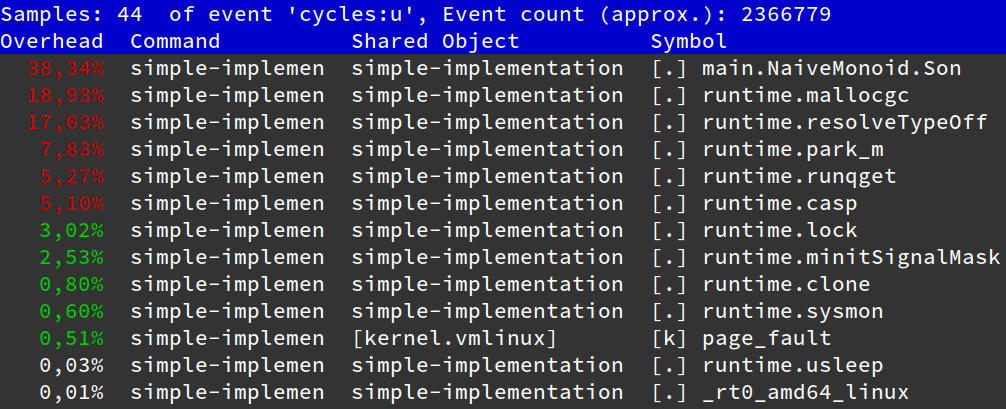
\includegraphics[scale=0.35]{perf.png}
	\caption{Informations présentées par l'écran principal de \texttt{perf}}
\end{figure}

Les statistiques de charge et le \emph{monitoring} des systèmes de calculs seront effectuées grâce au projet libre \texttt{netdata}\footnote{\url{http://my-netdata.io/}}. Cette application associe en effet des informations pertinentes (charge CPU, RAM, réseau, \dots) visualisable en temps réel à un impact sur la machine très faible. Elle sera utilisée pour contrôler les différentes données d'utilisation du système en fonction du temps et ainsi vérifier facilement le bon fonctionnement de la distribution.

\begin{figure}[h]
	\centering
	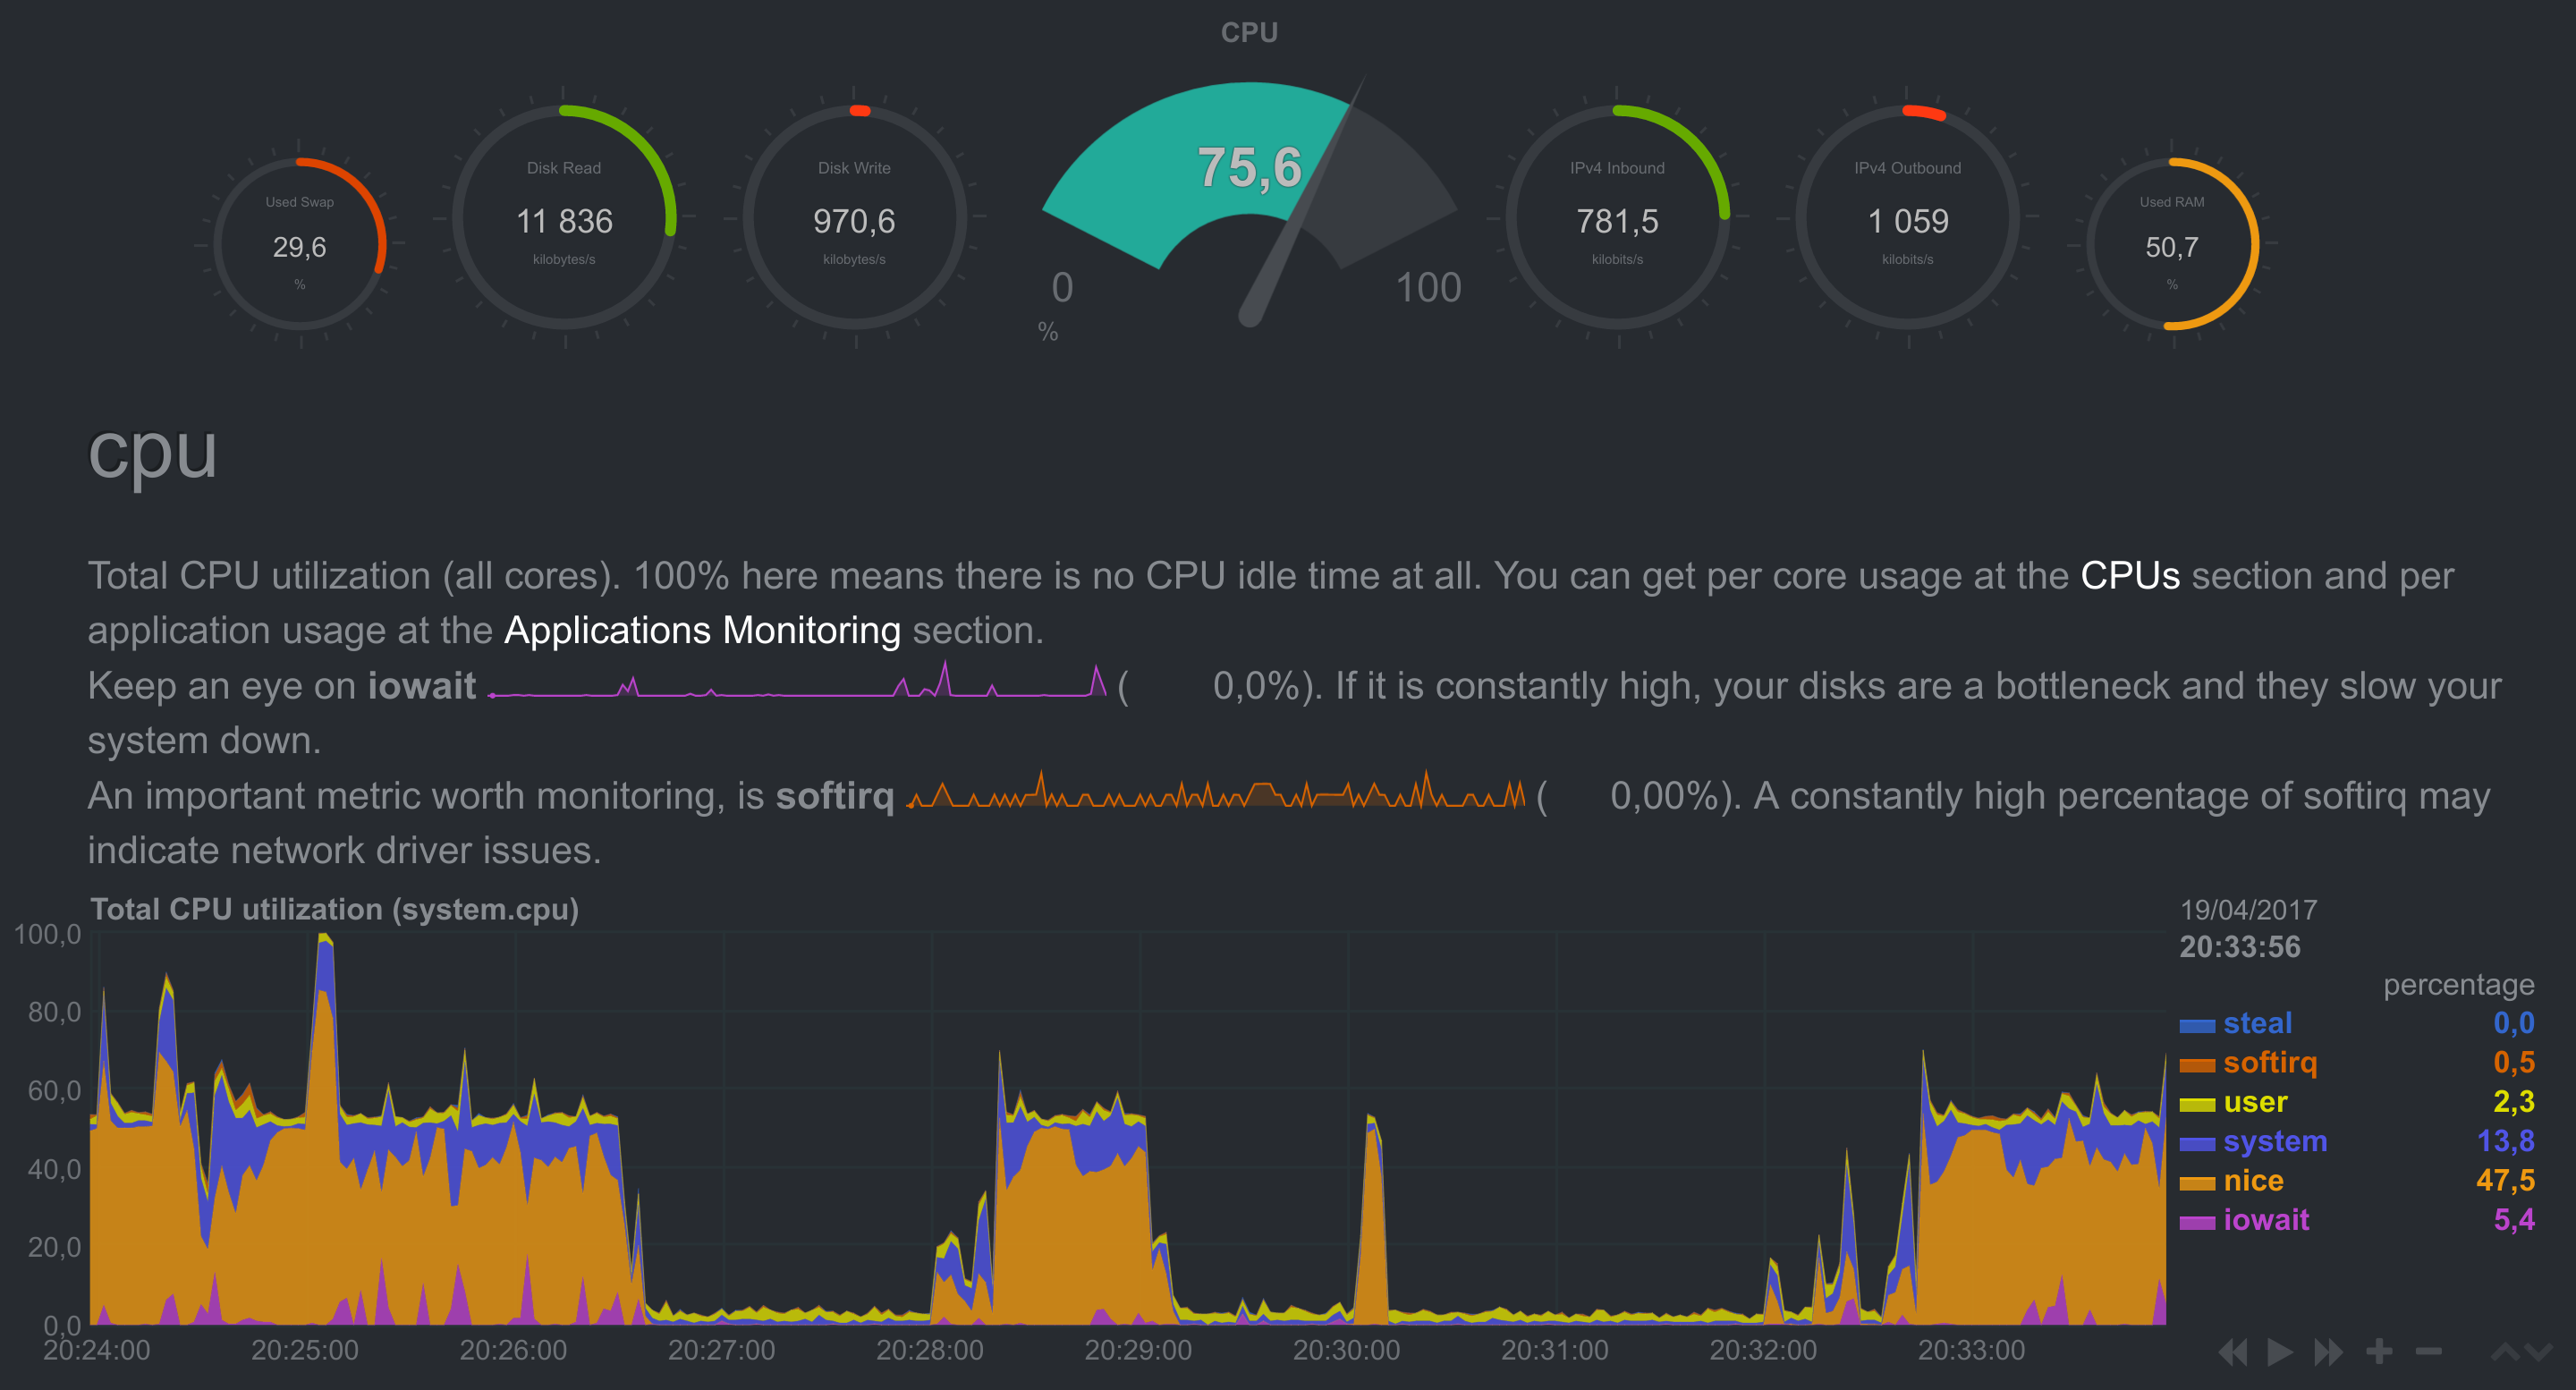
\includegraphics[scale=0.125]{netdata.png}
	\caption{Capture d'écran d'un panneau de contrôle de \texttt{netdata}}
\end{figure}

\section{Idée générale}
Pour résoudre et distribuer le problème, nous avons opté pour le rajout d'un ``étage'' dans l'architecture, lui aussi basé sur le vol de tâches.

Jusqu'à présent, Cilk effectuait un équilibrage local à la machine jusqu'à la profondeur définie par \texttt{STACK\_BOUND}. Dans la solution mise en \oe{}uvre, le programme de distribution effectue un vol de tâches mais cette fois ci sur le réseau, jusqu'à la profondeur \texttt{CILK\_BOUND} avant d'appeler \texttt{walk\_children()}.

Cette dernière va ensuite équilibrer localement jusqu'à \texttt{STACK\_BOUND} tandis que \texttt{walk\_children\_stack()} s'occupera des profondeurs supérieures, jusqu'à \texttt{MAX\_GENUS}.

La mise en place de cette solution a donc nécessité de pouvoir appeler les fonctions déjà implémentées en \texttt{C++}. Le langage Go n'étant pas prévu pour effectuer des optimisations bas niveau, j'ai pris la décision de réaliser des \emph{bindings}\footnote{Interface de programmation permettant d'appeler du code existant depuis un autre langage.} Go $\Leftrightarrow$ \texttt{C++}.

Ce développement a pris un certain temps dans le déroulement de ce TER car nous avons été confrontés à un bug de GCC qui sera abordé par la suite. De plus, j'ai fait le choix de mettre en place des tests unitaires\footnote{Tests automatisés portant sur une partie du code d'un programme et permettant notamment de vérifier, dans notre cas, que des résultats corrects sont bien retournés ou que des erreurs sont bien générées.} afin de ne pas me heurter à des incohérences de résultat par la suite. La mise en place de ces tests a également pris du temps.

L'intégration de la distribution par vol de tâches en Go a été plutôt simple à réaliser. En effet, le langage propose, notamment via les \emph{channels}\footnote{\url{https://gobyexample.com/select}}, différentes fonctionnalités très utiles à l'implémentation de notre système.

Je n'ai pas rencontré de difficultés non plus à implémenter la partie réseau, c'est à dire le code gérant les échanges de messages et les entités clients et serveurs. Le langage Go ayant été conçu, notamment par le biais de sa librairie standard, pour s'adapter facilement à la mise en place de protocoles de transfert ou de microservices\footnote{\url{https://fr.wikipedia.org/wiki/Microservices}}.

Cependant, la détection de la fin du calcul a été un challenge intéressant au niveau algorithmique. À l'heure où j'écris ce rapport, cela n'est pas encore au point et devrait être terminé avant de lancer les calculs définitifs.

\section{Organisation}
Le code s'articule autour d'un dépôt Git\footnote{\url{https://github.com/efournival/ter-lri}} qui contient tous les essais ainsi que la version finale destinée à être lancée sur un cluster de calcul.

Le dépôt contient plusieurs dossiers :
\begin{itemize}
	\item	\texttt{danse} : la version finale nommée DANSE pour \emph{Distributed Array of Numerical Semigroup Explorations}, soit en français un réseau distribué d'exploration de semigroupes numériques;
	\item	\texttt{go-numeric-monoid} : les \emph{bindings} Go de l'algorithme optimisé écrit en \texttt{C++};
	\item	\texttt{simple-implementation} : implémentation propre avec tests unitaires de l'algorithme naïf et de l'algorithme optimisé, non parallélisée;
\end{itemize}

\begin{figure}[h]
	\centering
	
\includegraphics[scale=0.35]{danse.png}
	\caption{Logo du programme de distribution \texttt{danse}, réalisé à partir du logo original du langage Go de Renee French}
\end{figure}

L'objectif est de lancer les calculs jusqu'au genre 70 sur des machines performantes. Ces résultats n'ont jamais été obtenus auparavant. Pour comparer, le calcul jusqu'au genre 67 sur une machine à 32 c\oe{}urs AMD a pris 18 jours \cite{exploring-ns}.

\section{Bug GCC Cilk n°80038}
Certaines méthodes de l'implémentation originale réalisée par Florent Hivert et Jean Fromentin font appel à du code spécifique très optimisé que seul certains compilateurs, ici GCC pour le langage C++, peuvent générer. C'est pour cela que des \emph{bindings} Go ont dû être implémentés afin de faire le lien entre le code généré par GCC et les fonctionnalités plus haut niveau (notamment côté réseau) du langage Go.

Ces \emph{bindings} ont été mis en place conjointement avec des tests unitaires. Ces derniers sont, en plus d'être fortement recommandés en général, omniprésents dans les développements réalisés en Go. En effet, le langage propose divers outils pour réaliser très simplement et rapidement ce genre de tests : la commande \texttt{go test}, le package \texttt{testing}, etc.

C'est donc dans ce cadre que je me suis rendu compte que les résultats (le comptage du nombre de semigroupes) renvoyés par les différentes explorations de l'arbre étaient incorrects, bien qu'aucune erreur ne soit remontée. Ces résultats incohérents sont également rencontrés avec le code original de \texttt{NumericMonoid}.

À la suite de nombreux tests, le problème a été identifié comme lié à la version du compilateur GCC. Ma machine de travail personnelle étant sous ArchLinux, je dispose de la dernière version stable (GCC 6) qui engendre ces résultats incorrects. Le développement de \texttt{NumericMonoid} ayant été réalisé à l'aide de GCC 5, les valeurs retournées étaient correctes jusque là.

Nous avons donc publié un rapport de bug avec un exemple réduit de code posant problème\footnote{\url{https://gcc.gnu.org/bugzilla/show_bug.cgi?id=80038}}. Le code minimal est visible en annexe \ref{anx:bugcilk}.

Il s'est avéré que GCC, depuis l'introduction d'un correctif concernant les arguments des lambda fonctions avec Cilk, appelait les destructeurs des arguments concernés au mauvais moment.

Mon encadrant, Florent Hivert, a rapidement trouvé une solution à ce problème une fois qu'il fut identifié : passer les semigroupes numériques par valeur et pas par référence. Cela implique une copie et grève les performances de l'ordre de 5\%. Heureusement, le bug a été résolu par Xi Ruoyao et le correctif sera mis en place dans la prochaine version mineure de GCC.

\chapter*{Conclusion}
\addcontentsline{toc}{chapter}{Conclusion}

À l'heure où j'écris ce rapport, nous n'avons aucune certitude concernant la fiabilité et l'efficacité du programme que j'ai développé. Celui-ci doit distribuer l'exploration de l'arbre des semigroupes numériques de manière correcte, c'est à dire en retournant le bon résultat, et performante afin de garder un bon facteur d'accélération. Tout cela sera vérifié le jeudi précédant la soutenance et nous devrions obtenir les résultats deux ou trois semaines plus tard.

Cependant, cela n'enlève rien au fait que ce TER a été très réussi en termes de compétences acquises et d'immersion dans le monde de la recherche. En effet, j'ai pu acquérir des connaissances dans des domaines variés comme l'optimisation, l'algorithmique, la parallélisation, etc.

Les différentes personnes que j'ai rencontré au LRI étaient toutes sympathiques et passionnées. J'ai apprécié cet aperçu de la partie recherche du métier d'enseignant-chercheur qui sévit à la faculté des sciences. Je remercie Florent Hivert pour avoir accepté de m'encadrer durant ce TER.

Je pense que le Travail d'Étude et de Recherche est un très bon moyen de faire découvrir le monde de la recherche aux étudiants tout en les impliquant sur un sujet qui les intéresse. Étant donné le travail que cela représente, un plus gros coefficient et peut-être plus de présence au laboratoire auraient été de vrais plus à la formation.

\printbibliography
\addcontentsline{toc}{chapter}{Bibliographie}

\chapter*{Annexes}
\addcontentsline{toc}{chapter}{Annexes}
\renewcommand{\thesection}{\Roman{section}}
\setcounter{section}{0}

\section{Déroulement}
\label{anx:deroulement}

\subsection*{Jeudi 12 janvier 2017}
Installation au LRI, explications :
\begin{itemize}
	\item	parcours de l'arbre de semigroupes numériques

	\item	structures de données utilisées, notamment dans \texttt{NumericMonoid}

	\item	algorithme ``naïf'' : tableau de booléens (le nombre est-il dans le semigroupe ?) de taille $B = 3 \cdot G - 1$ où G est le genre soit la profondeur dans l'arbre et le nombre de trous
			\begin{algorithmic}
				\FOR {$g \text{ de dernierEnlevé + 1 à } B$}
					\IF{$T[g]$}
						\FOR {$i \text{ de } 1 \text{ à } \lfloor \frac{g}{2} \rfloor$}
							\IF{$T[i] \land T[g-i]$}
								\STATE $g$ est une décomposition
							\ENDIF
						\ENDFOR
					\ENDIF
				\ENDFOR
			\end{algorithmic}

	\item	algorithme optimisé facilitant la vectorisation : tableau d'entiers modélisant le nom\-bre de paires ($i, j \in$ SN tel que $i + j = g$ et $i \leq j$), tous les nombres avec exactement une paire sont des générateurs
\end{itemize}

\subsection*{Autonomie}
\begin{itemize}
	\item	première implémentation de l'algorithme naïf; difficultés : initialisation, confusion décomposition/générateur
	\item	première implémentation de l'algorithme optimisé
	\item	organisation du dépôt Git
\end{itemize}

\subsection*{Lundi 16 janvier 2017}
\begin{itemize}
	\item	mise au point et correction de l'algorithme naïf
	\item	débogage et tests
\end{itemize}

\subsection*{Autonomie}
\begin{itemize}
	\item	mise en place de tests unitaires
	\item	amélioration de l'algorithme naïf; difficulté : les tests unitaires sur des semigroupes connus passent, mais le résultat final (nombre de semigroupes calculés, par genre) n'est pas bon
	\item	correction de l'algorithme optimisé : il fonctionne
	\item	correction de l'algorithme naïf en rajoutant l'attribut \texttt{m}
	\item	parallélisation à l'aide d'un verrou partagé sur la pile (\texttt{sync.RWMutex}) et d'une incrémentation atomique sur les cellules du tableau de résultat (packages \texttt{sync/atomic} et \texttt{unsafe})
	\item	difficultés : critère d'arrêt pour un genre donné, profiler le code car la charge processeur reste faible (verrous ?), types de données, stratégies de parallélisation
\end{itemize}

\subsection*{Jeudi 26 janvier 2017}
\begin{itemize}
	\item	présentation du profiling avec la commande \texttt{perf}, elle est effective au niveau hardware donc ne dégrade pas les performances; permet d'associer code machine et symboles de débogage au temps relatif passé par le processeur; commandes \texttt{perf record}, \texttt{perf report} et \texttt{sudo perf top} pour du temps réel
	\item	pour tester \texttt{NumericMonoid}, on ferra attention à se positionner dans le répertoire \texttt{src/Cilk++}
	\item	il faut vérifier la bonne parallélisation en testant différents nombres de threads (modification de \texttt{runtime.GOMAXPROCS}); une bonne parallélisation donnera le résultat deux fois plus rapidement si on double le nombre de threads (jusqu'au nombre de c\oe{}urs, mais attention à l'HyperThreading : tester avec 2 fois le nombre de c\oe{}urs physiques); seul 5 à 10\% du temps de calcul total est destiné à la communication/synchronisation
	\item	pour remplacer l'utilisation de \texttt{sync/atomic}, on peut utiliser un stockage local au thread; implémenté dans Sage en Python; en Go, on pourra utiliser des \emph{channels} (\emph{pipes} en Python)
	\item	pour s'arrêter lorsque les calculs sont parallélisés : compter le nombre de processus actifs (entre le pop de la pile et après les push); on a fini lorsque la pile est vide et qu'il n'y a plus aucun processus actif; fait appel à \texttt{sync/atomic}
\end{itemize}

\subsection*{Jeudi 2 février 2017}
\begin{itemize}
	\item	profiling en utilisant \verb|perf| : mise en évidence de délais supplémentaires induits par les communications et la synchronisation
	\item	mise en place d'un arrêt ``propre'' avec comptage du nombre de routines actives et de l'état de la pile
	\item	les threads de l'ordonnanceur interne du Go (autant de threads que de cœurs logiques) ne prennent 100\% de la charge processeur : mise en évidence (de trop) d'attente de verrous
\end{itemize}

\subsection*{Autonomie}
\begin{itemize}
	\item	réflexion sur une stratégie de parallélisation qui ne nécessite pas de verrous et qui permettra à terme de mettre en place le calcul distribué
	\item	rédaction du rapport
	\item	difficultés sur la multiplicité, le conducteur, la méthode pour compter les combinaisons dans l'algorithme optimisé
\end{itemize}

\subsection*{Mercredi 8 février 2017}
\begin{itemize}
	\item	éclaircissements sur les nombres de décomposition, les générateurs, le conducteur, la multiplicité, \dots
	\item	discussion sur la stratégie à adopter pour la distribution : faire appel au code \texttt{C++} multithreadé à l'aide de \texttt{cgo} et gérer la distribution ainsi que le vol de tâche à l'aide d'un code Go natif
	\item	code à étudier : l'itérateur dans \texttt{treewalk.cpp} de \texttt{NumericMonoid} ainsi que la méthode \texttt{walk\_children\_stack}
	\item	pistes pour l'implémentation du vol de tâches : documentation automatique du code Python ainsi que le code source du projet Sage dans \path{src/sage/parallel/mapreduce.py}
\end{itemize}

\subsection*{Autonomie}
\begin{itemize}
	\item	rédaction du rapport : algorithmes, exemple de semigroupe et avancement
	\item	documentation et réflexion sur l'utilisation de \texttt{cgo}
	\item	découverte de \texttt{go build -gcflags='-m'} qui indique si des fonctions ont été ou pas inlinées, et pour quelles raisons
	\item	mise en place d'un package Go permettant de faire le lien entre le code optimisé de \texttt{NumericMonoid} et un code écrit en Go : implémentation d'une interface \texttt{C} $\Leftrightarrow$ \texttt{C++} pour pouvoir utiliser \texttt{cgo}
	\item	problèmes rencontrés : \texttt{NumericMonoid} fait une erreur de segmentation pour des valeurs de \texttt{MAX\_GENUS} inférieure à 16; sous GCC 6, les résultats (nombre de semigroupes par genre) diffèrent (!), résolu en forçant l'utilisation de GCC 5
\end{itemize}

\subsection*{Jeudi 2 mars 2017}
\begin{itemize}
	\item	il est ``normal'' que le programme fasse une erreur de segmentation pour une valeur de \texttt{MAX\_GENUS} $\leq 11$ car il s'agit d'une constante codée en dur et utilisée pour indiquer quelles explorations doivent être explorées par Cilk ou par dérécursivation (ligne 48 de \texttt{treewalk.cpp})
	\item	un bug a sûrement été introduit par la version 6 de GCC au niveau de la vérification des indices d'accès aux tableaux : des avertissements apparaissent à la compilation lorsque l'indice est non signé (type \texttt{ind\_t}), il n'y a plus d'avertissement si on change le \texttt{typedef} de \texttt{ind\_t} en quelque chose de signé
	\item	on veut vérifier que le Go supporte bien le modèle fork-join récursif, pour cela il faut implémenter l'exemple de Wikipédia (page anglaise) qui effectue un tri fusion
	\item	la suite du travail consistera à traduire en Go la boucle principale du code source original de \texttt{NumericMonoid} soit \texttt{walk\_children} ligne 49 de \texttt{treewalk.cpp}
\end{itemize}

\subsection*{Autonomie}
\begin{itemize}
	\item	nettoyage du dépôt et mise au propre des versions naïves et optimisées afin d'uniformiser les tests
	\item	mise en place d'une VM et lancement de la compilation sous GCC 7 afin de déterminer si le problème de résultats faux était toujours présent : c'est le cas
	\item	implémentation en Go de la boucle principale
\end{itemize}

\subsection*{Jeudi 9 mars}
\begin{itemize}
	\item	débogage du bug affectant les versions de GCC $\geq$ 6, découverte d'un correctif qui consiste à passer le monoïde à explorer par valeur plutôt que par référence, isolation du bug
	\item	suite de l'implémentation de la boucle principale : ajout de \emph{bindings} supplémentaires
\end{itemize}

\subsection*{Autonomie}
\begin{itemize}
	\item	le bug\footnote{\url{https://gcc.gnu.org/bugzilla/show_bug.cgi?id=80038}} est remonté à l'équipe de GCC, à première vue il s'agit d'un mauvais appel des destructeurs dans la fonction parent ce qui conduit à un accès sur pointeur nul dans la fonction fille (lancée via \texttt{cilk\_spawn})\footnote{\url{https://gcc.gnu.org/ml/gcc-help/2017-03/msg00037.html}}
	\item	mise en place du \emph{workflow} Go ainsi que du code haut niveau dans \texttt{danse}
	\item	suite de l'implémentation de la boucle principale : cela prend du temps à cause de la mise en place des \emph{bindings} Go, de la traduction du typage et des tests unitaires
	\item	finalisation de l'intégration continue
\end{itemize}

\subsection*{Jeudi 23 mars}
\begin{itemize}
	\item	présentation\footnote{\url{http://stackoverflow.com/questions/42816920/data-race-in-cilk-home-made-reducer}} du problème de \emph{race condition} dans Cilk
	\item	explications sur les différents niveaux de l'exploration de l'arbre : Cilk, instruction \texttt{popcount}, etc.
	\item	confirmation que l'ordonnanceur de Go est adapté à notre problème : pas d'explosion de la mémoire allouée ou de ralentissement quand un grand nombre de goroutines sont lancées
	\item	évaluation des performances de l'ordonnanceur de Go et des channels : moins bien que Cilk et du C++ optimisé mais satisfaisant
	\item	suite des opérations : distribuer le lancement des goroutines
\end{itemize}

\subsection*{Autonomie}
\begin{itemize}
	\item	réflexion sur la possible utilisation d'un algorithme de \emph{machine learning} pour ajuster et optimiser les différents paramètres au fur et à mesure du calcul
	\item	implémentation du système distribué
	\item	\emph{refactoring} du problème pour utiliser les fonctionnalités de synchronisation de Go : l'utilisation des \emph{channels} afin d'obtenir un calcul complètement asynchrone donne de bonnes performances et permet de très facilement mettre en place le vol de tâche et la couche réseau
\end{itemize}

\subsection*{Jeudi 6 avril}
\begin{itemize}
	\item	pas d'intérêt particulier à utiliser un algorithme de machine learning, on insistera par contre sur le choix des paramètres initiaux
	\item	attention à l'architecture basée entièrement sur des channels, les communications pour éviter les erreurs liées à la concurrence sont couteuses
	\item	mise au point sur les différents étages de l'arbre, on va tester dans un premier temps une constante \texttt{CILK\_BOUND}
	\item	informations sur le rendu du rapport : vers mi Avril, bien introduire le problème, mettre un dessin des différents étages de parallélisation/distribution
\end{itemize}

\subsection*{Autonomie}
\begin{itemize}
	\item	développement du programme de distribution final (DANSE)
	\item	mise en place sur la machine du centre de calcul de l'université \texttt{gocilk}
\end{itemize}

\subsection*{Jeudi 20 avril}
\begin{itemize}
	\item	relecture et correction du rapport
	\item	configuration de \texttt{gocilk} afin d'ouvrir les ports nécessaires à \texttt{netdata} et à \texttt{danse}
\end{itemize}

\newpage

\section{Code minimal causant le bug Cilk}
\label{anx:bugcilk}

\begin{verbatim}
#include <vector>
#include <cilk/cilk.h>

void walk(std::vector<int> v, unsigned size) {
  if (v.size() < size)
    for (int i=0; i<8; i++) {
      std::vector<int> vnew(v);
      vnew.push_back(i);
      cilk_spawn walk(vnew, size);
    }
}

int main(int argc, char **argv) {
  std::vector<int> v{};
  walk(v, 5);
}
\end{verbatim}

À compiler à l'aide de :

{\centering \texttt{g++-6 -std=c++11 -fcilkplus -g -Wall -lcilkrts red2.cpp -o red2}}

\end{document}
